
%%--------------------------------------------------
%% Serway: Physics for Scientists and Engineers
%%--------------------------------------------------


%% Chapter 12: Static Equilibrium and Elasticity
%%--------------------------------------------------


%% Table of Contents
%%--------------------------------------------------

%% 12.1 The Rigid Object in Equilibrium
%% 12.2 More on the Center of Gravity
%% 12.3 Examples of Rigid Objects in Static
%% 12.4 Equilibrium
%% 12.5 Elastic Properties of Solids


%% Serway Multiple Choice Questions
%%--------------------------------------------------
\element{serway-mc}{
\begin{question}{serway-ch12-q01}
    A uniform ladder \SI{15}{\foot} long is leaning against a frictionless wall at an angle of \ang{53} above the horizontal.
    The weight of the ladder is \SI{30}{\pound}.
    A \SI{75}{\pound} boy climbs \SI{6.0}{\foot} up the ladder.
    What is the magnitude of the friction force exerted on the ladder by the floor?
    \begin{multicols}{3}
    \begin{choices}
        \wrongchoice{\SI{43}{\pound}}
      \correctchoice{\SI{34}{\pound}}
        \wrongchoice{\SI{38}{\pound}}
        \wrongchoice{\SI{47}{\pound}}
        \wrongchoice{\SI{24}{\pound}}
    \end{choices}
    \end{multicols}
\end{question}
}

\element{serway-mc}{
\begin{question}{serway-ch12-q02}
    A horizontal meter stick supported at the \SI{50}{\centi\meter} mark has a mass of \SI{0.50}{\kilo\gram} hanging from it at the \SI{20}{\centi\meter} mark and a \SI{0.30}{\kilo\gram} mass hanging from it at the \SI{60}{\centi\meter} mark.
    Determine the position on the meter stick at which one would hang a third mass of \SI{0.60}{\kilo\gram} to keep the meter stick balanced.
    \begin{multicols}{3}
    \begin{choices}
        \wrongchoice{\SI{74}{\centi\meter}}
      \correctchoice{\SI{70}{\centi\meter}}
        \wrongchoice{\SI{65}{\centi\meter}}
        \wrongchoice{\SI{86}{\centi\meter}}
        \wrongchoice{\SI{62}{\centi\meter}}
    \end{choices}
    \end{multicols}
\end{question}
}

\element{serway-mc}{
\begin{question}{serway-ch12-q03}
    The figure shows a uniform,
        horizontal beam (length = \SI{10}{\meter}, mass = \SI{25}{\kilo\gram}) that is pivoted at the wall,
        with its far end supported by a cable that makes an angle of \ang{51} with the horizontal.
    \begin{center}
    \begin{tikzpicture}
        %% ceiling and wall
        \draw[thick] (0,-1) -- (0,6) -- (7,6);
        \node[anchor=east,fill,pattern=north east lines,minimum width=0.1cm, minimum height=7cm] at (0,2.5) {};
        \node[anchor=south,fill,pattern=north east lines,minimum width=7.2cm, minimum height=0.1cm] at (3.4,6) {};
        %% hinge and rod
        \draw (0.1,0) circle (0.1);
        \draw[fill=white!90!black] (0.2,-0.1) rectangle (6,0.1);
        %% Man
        \begin{scope}[anchor=south,shift={(1.8,0.1)},scale=1.5]
            \draw[thick] (0,0.25) -- (0,0.75);
            %% Legs
            \draw[thick] (0,0.25) -- (-0.25,0);
            \draw[thick] (0,0.25) -- (+0.25,0);
            %% Arms
            \draw[thick] (0,0.50) -- (-0.25,0.55);
            \draw[thick] (0,0.50) -- (+0.25,0.55);
            %% Head
            \draw[fill=white!90!black] (0,0.80) circle (0.15cm);
        \end{scope}
        %% distance
        \draw[thick,<->] (0,2) -- (1.8,2) node[pos=0.5,anchor=center,fill=white] {\SI{3.0}{\meter}};
        \draw[thick,<->] (0,-0.5) -- (6,-0.5) node[pos=0.5,anchor=center,fill=white] {\SI{10.0}{\meter}};
        %% Cable
        \draw[thick] (6,0.1) -- (1.22,6);
        \draw[<->] (4.5,0.1) arc (180:129:1.5) node[pos=0.5,anchor=east] {\ang{51}};
    \end{tikzpicture}
    \end{center}
    If a person (mass = \SI{60}{\kilo\gram}) stands \SI{3.0}{\meter} from the pivot,
        what is the tension in the cable?
    \begin{multicols}{3}
    \begin{choices}
        \wrongchoice{\SI{0.83}{\kilo\newton}}
        \wrongchoice{\SI{0.30}{\kilo\newton}}
      \correctchoice{\SI{0.39}{\kilo\newton}}
        \wrongchoice{\SI{0.42}{\kilo\newton}}
        \wrongchoice{\SI{3.0}{\kilo\newton}}
    \end{choices}
    \end{multicols}
\end{question}
}

\element{serway-mc}{
\begin{question}{serway-ch12-q04}
    A uniform \SI{100}{\pound} beam is held in a vertical position by a pin at its lower end and a cable at its upper end.
    A horizontal force (magnitude $P$) acts as shown in the figure.
    \begin{center}
    \begin{tikzpicture}[scale=0.4]
        %% Floor
        \draw (0,8) -- (-13.85,0) -- (3,0);
        \node[anchor=north,fill,pattern=north east lines,minimum width=8cm, minimum height=0.1cm] at (-5.5,0) {};
        \draw[<->] (-13.85,0) ++(0:4) arc(0:30:4) node[pos=0.5,anchor=west] {\ang{30}};
        %% hinge
        \draw[thick] (0,0.2) circle (0.2cm);
        \draw[fill=white!80!black] (-0.2,0.4) rectangle (0.2,8);
        %% five and three feet
        \draw[dashed] (0,8) -- (2.5,8);
        \draw[thick,<->] (+2,0) -- (+2,4.9) node[pos=0.5,anchor=center,fill=white] {\SI{5.0}{\foot}};
        \draw[thick,<->] (+2,5.1) -- (+2,8) node[pos=0.5,anchor=center,fill=white] {\SI{3.0}{\foot}};
        %% Force P
        \draw[ultra thick,->] (0,5) -- (4,5) node[pos=0.75,anchor=south] {$P$};
    \end{tikzpicture}
    \end{center}
    If $P=\SI{75}{\pound}$, what is the tension in the cable?
    \begin{multicols}{3}
    \begin{choices}
      \correctchoice{\SI{54}{\pound}}
        \wrongchoice{\SI{69}{\pound}}
        \wrongchoice{\SI{47}{\pound}}
        \wrongchoice{\SI{61}{\pound}}
        \wrongchoice{\SI{75}{\pound}}
    \end{choices}
    \end{multicols}
\end{question}
}

\element{serway-mc}{
\begin{question}{serway-ch12-q05}
    A \SI{25}{\foot} long crane supported at its lower end by a pin is elevated by a horizontal cable as shown in the figure.
    A \SI{250}{\pound} load is suspended from the outer end of the crane.
    \begin{center}
    \begin{tikzpicture}
        %% Wall
        \node[anchor=east,fill,pattern=north east lines,minimum width=0.1cm, minimum height=5cm] at (0,1.5) {};
        \draw (0,-1) -- (0,4);
        %% hinge and rod
        \draw (0.1,0) circle (0.1);
        \draw[fill=white!90!black,rotate around={30:(0.1,0)}] (0.2,-0.1) rectangle (6,0.1);
        \draw[<->] (0,2.115) arc (90:30:2) node[pos=0.5,anchor=center,fill=white] {\ang{60}};
        %% Weight
        \node[draw,fill=white!90!black,anchor=north,minimum size=1.5cm,rounded corners=0.5ex] (M) at (5.3,1) {\SI{250}{\pound}};
        %% Rope and/or cable
        \draw[very thick] (0,3) -- (5.16,3.04) -- ++(-60:0.2) -- (M.north);
    \end{tikzpicture}
    \end{center}
    The center of gravity of the crane is \SI{10}{\foot} from the pin,
        and the crane weighs \SI{200}{\pound}.
    What is the tension in the horizontal cable?
    \begin{multicols}{3}
    \begin{choices}
        \wrongchoice{\SI{610}{\pound}}
        \wrongchoice{\SI{540}{\pound}}
        \wrongchoice{\SI{640}{\pound}}
      \correctchoice{\SI{570}{\pound}}
        \wrongchoice{\SI{2000}{\pound}}
    \end{choices}
    \end{multicols}
\end{question}
}

\element{serway-mc}{
\begin{question}{serway-ch12-q06}
    A uniform beam having a mass of \SI{60}{\kilo\gram} and a length of \SI{2.8}{\meter} is held in place at its lower end by a pin.
    Its upper end leans against a vertical frictionless wall as shown in the figure.
    \begin{center}
    \begin{tikzpicture}
        %% Wall and Floor
        \draw (0,0) -- (6,0);
        \node[anchor=north,fill,pattern=north east lines,minimum width=6.0cm, minimum height=0.05cm] at (3,0) {};
        \draw (0,0) -- (0,5);
        \node[anchor=east,fill,pattern=north east lines,minimum width=0.05cm, minimum height=5.2cm] at (0,2.4) {};
        %% hinge and rod
        \draw[fill=white!80!black] (5,0.1) circle (0.1);
        \draw[fill=white!40!black] (5,0.1) circle (0.05);
        \draw[fill=white!90!black,rotate around={50:(5,0.1)}] (4.9,0.2) rectangle (5.1,6.52);
        %% angle
        \draw[<->] (3.4,0) arc (180:140:1.5) node[pos=0.5,anchor=center,fill=white] {\ang{40}};
    \end{tikzpicture}
    \end{center}
    What is the magnitude of the force the pin exerts on the beam?
    \begin{multicols}{2}
    \begin{choices}
      \correctchoice{\SI{0.68}{\kilo\newton}}
        \wrongchoice{\SI{0.57}{\kilo\newton}}
        \wrongchoice{\SI{0.74}{\kilo\newton}}
        \wrongchoice{\SI{0.63}{\kilo\newton}}
        \wrongchoice{\SI{0.35}{\kilo\newton}}
    \end{choices}
    \end{multicols}
\end{question}
}

\element{serway-mc}{
\begin{question}{serway-ch12-q07}
    A uniform \SI{120}{\pound} beam is supported in a horizontal position by a pin and cable as shown in the figure.
    \begin{center}
    \begin{tikzpicture}
        %% ceiling and wall
        \draw[thick] (0,-1) -- (0,6) -- (7,6);
        \node[anchor=east,fill,pattern=north east lines,minimum width=0.1cm, minimum height=7cm] at (0,2.5) {};
        \node[anchor=south,fill,pattern=north east lines,minimum width=7.2cm, minimum height=0.1cm] at (3.4,6) {};
        %% hinge and rod
        \draw[fill=white!80!black] (0.1,0) circle (0.1);
        \draw[fill=white!40!black] (0.1,0) circle (0.05);
        \draw[fill=white!90!black] (0.2,-0.1) rectangle (6,0.1);
        %% distance
        \draw[thick,<->] (0,-0.5) -- (6,-0.5) node[pos=0.5,anchor=center,fill=white] {\SI{12}{\foot}};
        %% Cable
        \draw[dashed] (6,0.1) -- ++(90:3);
        \draw[very thick] (6,0.1) -- (1.55,6);
        \draw[<->] (6,2) arc (90:127:1.9) node[pos=0.5,anchor=south] {\ang{37}};
    \end{tikzpicture}
    \end{center}
    What is the magnitude of the force by the pin on the beam?
    \begin{multicols}{3}
    \begin{choices}
        \wrongchoice{\SI{94}{\pound}}
        \wrongchoice{\SI{88}{\pound}}
        \wrongchoice{\SI{63}{\pound}}
      \correctchoice{\SI{75}{\pound}}
        \wrongchoice{\SI{150}{\pound}}
    \end{choices}
    \end{multicols}
\end{question}
}

\element{serway-mc}{
\begin{question}{serway-ch12-q08}
    A \SI{20}{\meter} long steel wire
        (cross-section \SI{1}{\centi\meter\squared}, Young’s modulus \SI{2e11}{\newton\per\meter\squared}),
        is subjected to a load of \SI{25 000}{\newton}.
    How much will the wire stretch under the load?
    \begin{multicols}{3}
    \begin{choices}
        \wrongchoice{\SI{0.25}{\centi\meter}}
      \correctchoice{\SI{2.5}{\centi\meter}}
        \wrongchoice{\SI{12.5}{\centi\meter}}
        \wrongchoice{\SI{25}{\centi\meter}}
        \wrongchoice{\SI{1.25}{\centi\meter}}
    \end{choices}
    \end{multicols}
\end{question}
}

\element{serway-mc}{
\begin{question}{serway-ch12-q09}
    How large a force is necessary to stretch a \SI{2}{\milli\meter} diameter copper wire $\left(Y=\SI{11e10}{\newton\per\meter\squared}\right)$ by \SI{1}{\percent}?
    \begin{multicols}{2}
    \begin{choices}
        \wrongchoice{\SI{2163}{\newton}}
      \correctchoice{\SI{3455}{\newton}}
        \wrongchoice{\SI{6911}{\newton}}
        \wrongchoice{\SI{11146}{\newton}}
        \wrongchoice{\SI{5240}{\newton}}
    \end{choices}
    \end{multicols}
\end{question}
}

\element{serway-mc}{
\begin{question}{serway-ch12-q10}
    How large a pressure increase (in \si{\atm}) must be applied to water if it is to be compressed in volume by \SI{1}{\percent}?
    The bulk modulus of water is \SI{2e9}{\newton\per\meter\squared} and $\SI{1}{\atm}=\SI{e5}{\newton\per\meter\squared}$.
    \begin{multicols}{2}
    \begin{choices}
        \wrongchoice{\SI{50}{\atm}}
        \wrongchoice{\SI{100}{\atm}}
        \wrongchoice{\SI{1 080}{\atm}}
        \wrongchoice{\SI{400}{\atm}}
      \correctchoice{\SI{200}{\atm}}
    \end{choices}
    \end{multicols}
\end{question}
}

\element{serway-mc}{
\begin{questionmult}{serway-ch12-q11}
    The diagrams below show forces applied to a wheel that weighs \SI{20}{\newton}.
    The symbol $\mathbf{W}$ stands for the weight.
    In which diagram(s) is the wheel in equilibrium?
    \begin{multicols}{2}
    \begin{choices}
        %% NOTE: questionmult, due to diagram(s) above
        \AMCboxDimensions{down=-1.5cm}
        \wrongchoice{
            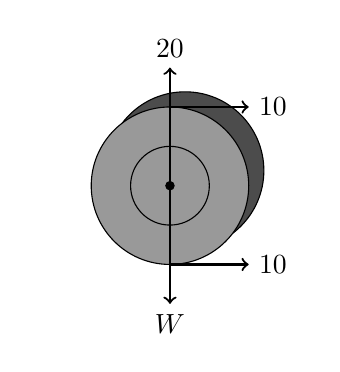
\begin{tikzpicture}
                \draw[white] (-1.8,-2) rectangle (1.8,2);
                %% inner and outer circle
                \draw[fill=white!30!black] (0,0,-0.5) circle (1.0);
                \draw[fill=white!60!black] (0,0) circle (1.0);
                \draw (0,0) circle (0.5);
                \draw[fill] (0,0) circle (1.5pt);
                %% forces
                \draw[thick,->] (0,0) -- ++(90:1.5) node[anchor=south] {\SI{20}{\newton}};
                \draw[thick,->] (0,0) -- ++(270:1.5) node[anchor=north] {$W$};
                \draw[thick,->] (0,+1) -- ++(0:1) node[anchor=west] {\SI{10}{\newton}};
                \draw[thick,->] (0,-1) -- ++(0:1) node[anchor=west] {\SI{10}{\newton}};
            \end{tikzpicture}
        }
        \wrongchoice{
            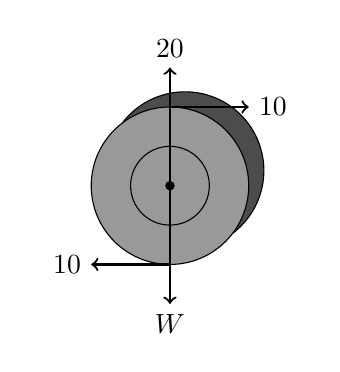
\begin{tikzpicture}
                \draw[white] (-1.8,-2) rectangle (1.8,2);
                %% inner and outer circle
                \draw[fill=white!30!black] (0,0,-0.5) circle (1.0);
                \draw[fill=white!60!black] (0,0) circle (1.0);
                \draw (0,0) circle (0.5);
                \draw[fill] (0,0) circle (1.5pt);
                %% forces
                \draw[thick,->] (0,0) -- ++(90:1.5) node[anchor=south] {\SI{20}{\newton}};
                \draw[thick,->] (0,0) -- ++(270:1.5) node[anchor=north] {$W$};
                \draw[thick,->] (0,+1) -- ++(0:1) node[anchor=west] {\SI{10}{\newton}};
                \draw[thick,->] (0,-1) -- ++(180:1) node[anchor=east] {\SI{10}{\newton}};
            \end{tikzpicture}
        }
        %% ANS is C
        \correctchoice{
            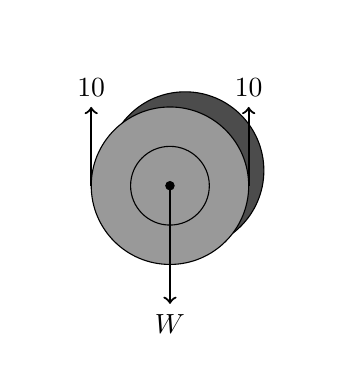
\begin{tikzpicture}
                \draw[white] (-1.8,-2) rectangle (1.8,2);
                %% inner and outer circle
                \draw[fill=white!30!black] (0,0,-0.5) circle (1.0);
                \draw[fill=white!60!black] (0,0) circle (1.0);
                \draw (0,0) circle (0.5);
                \draw[fill] (0,0) circle (1.5pt);
                %% forces
                \draw[thick,->] (0,0) -- ++(270:1.5) node[anchor=north] {$W$};
                \draw[thick,->] (+1,0) -- ++(90:1) node[anchor=south] {\SI{10}{\newton}};
                \draw[thick,->] (-1,0) -- ++(90:1) node[anchor=south] {\SI{10}{\newton}};
            \end{tikzpicture}
        }
        \wrongchoice{
            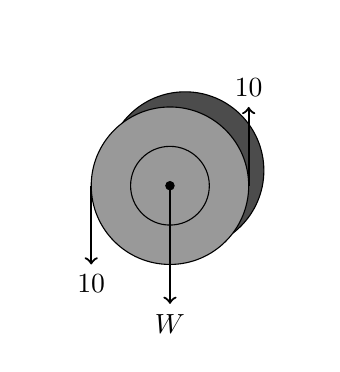
\begin{tikzpicture}
                \draw[white] (-1.8,-2) rectangle (1.8,2);
                %% inner and outer circle
                \draw[fill=white!30!black] (0,0,-0.5) circle (1.0);
                \draw[fill=white!60!black] (0,0) circle (1.0);
                \draw (0,0) circle (0.5);
                \draw[fill] (0,0) circle (1.5pt);
                %% forces
                \draw[thick,->] (0,0) -- ++(270:1.5) node[anchor=north] {$W$};
                \draw[thick,->] (+1,0) -- ++(90:1) node[anchor=south] {\SI{10}{\newton}};
                \draw[thick,->] (-1,0) -- ++(270:1) node[anchor=north] {\SI{10}{\newton}};
            \end{tikzpicture}
        }
    \end{choices}
    \end{multicols}
\end{questionmult}
}

%\element{serway-mc}{
%\begin{question}{serway-ch12-q12}
%    The diagrams below show forces of magnitude $F$ applied to an equilateral triangular block of uniform thickness.
%    In which diagram(s) is the block in equilibrium?
%    \begin{multicols}{2}
%    \begin{choices}
%        \AMCboxDimensions{down=-1.5cm}
%        \wrongchoice{
%            \begin{tikzpicture}
%                \draw[fill] (0,0,0) circle (1.5pt);
%                %\draw[fill=white!90!black] (0,1,0.5) -- (-0.866,-0.5,0.5) -- (0.866,-0.5,0.5) -- cycle;
%                \draw[fill=white!90!black] (0,1,0) -- (-0.866,-0.5,0) -- (0.866,-0.5,0) -- cycle;
%                \draw[fill=white!90!black] (0,1,0) -- (0,1,1) -- (-0.855,-0.5,1) -- (-0.855,-0.5,0) -- cycle;
%                \draw[fill=white!90!black] (-0.855,-0.5,0) -- (-0.855,-0.5,1) -- (0.866,-0.5,1) -- (0.866,-0.5,0) -- cycle;
%                %\draw[fill=white!90!black] (-0.855,+0.5,0) -- (-0.855,+0.5,0.5);
%                %% vectors
%                \draw[very thick,->] (0,1) -- ++(60:0.5);
%                \draw[very thick,->] (-0.866,-0.5) -- ++(180:0.5);
%                \draw[very thick,->] (+0.866,-0.5) -- ++(300:0.5);
%                %% NOTE: diagram is just nine lines, one cirlce and three arrow!!
%            \end{tikzpicture}
%        }
%        %% NOTE: ans is B
%    \end{choices}
%    \end{multicols}
%\end{question}
%}

\newcommand{\serwayChTwelveQThirteen}{
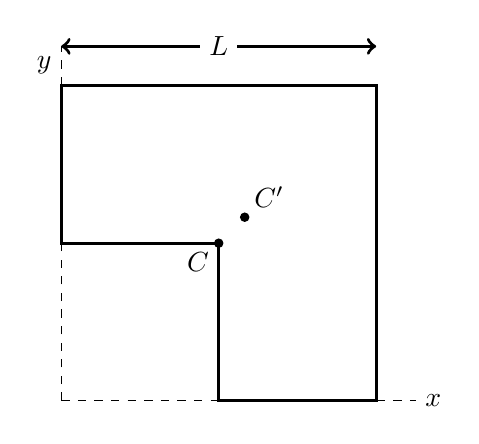
\begin{tikzpicture}
    %% Rigid Mass
    \draw[very thick] (0,2) -- (0,4) -- (4,4) -- (4,0) -- (2,0) -- (2,2) -- cycle;
    %% Center
    \draw[fill] (2,2) circle (1.5pt) node[anchor=north east] {$C$};
    \draw[fill] (2.33,2.33) circle (1.5pt) node[anchor=south west] {$C^{\prime}$};
    %% Labels
    \draw[very thick,<->] (0,4.5) -- (4,4.5) node[anchor=center,pos=0.5,fill=white] {$L$};
    %% Removed mass and Axis Labels
    \draw[dashed] (0,0) -- (4.5,0) node[anchor=west] {$x$};
    \draw[dashed] (0,0) -- (0,4.5) node[anchor=north east] {$y$};
\end{tikzpicture}
}

\element{serway-mc}{
\begin{question}{serway-ch12-q13}
    A square of side $\frac{L}{2}$ is removed from one corner of a square sandwich that has sides of length $L$.
    The center of mass of the remainder of the sandwich moves from $C$ to $C^{\prime}$.
    \begin{center}
        \serwayChTwelveQThirteen
    \end{center}
    The displacement of the $x$ coordinate of the center of mass (from $C$ to $C^{\prime}$) is:
    \begin{multicols}{3}
    \begin{choices}
      \correctchoice{$\dfrac{1}{12}L$}
        \wrongchoice{$\dfrac{\sqrt{2}}{12}L$}
        \wrongchoice{$\dfrac{1}{6}L$}
        \wrongchoice{$\dfrac{1}{8}L$}
        \wrongchoice{$\dfrac{\sqrt{2}}{8}L$}
    \end{choices}
    \end{multicols}
\end{question}
}

\element{serway-mc}{
\begin{question}{serway-ch12-q14}
    A square of side $\frac{L}{2}$ is removed from one corner of a square sandwich that has sides of length $L$.
    The center of mass of the remainder of the sandwich moves from $C$ to $C^{\prime}$.
    \begin{center}
        \serwayChTwelveQThirteen
    \end{center}
    The displacement of the $y$ coordinate of the center of mass (from $C$ to $C^{\prime}$) is:
    \begin{multicols}{3}
    \begin{choices}
      \correctchoice{$\dfrac{1}{12}L$}
        \wrongchoice{$\dfrac{\sqrt{2}}{12}L$}
        \wrongchoice{$\dfrac{1}{6}L$}
        \wrongchoice{$\dfrac{1}{8}L$}
        \wrongchoice{$\dfrac{\sqrt{2}}{8}L$}
    \end{choices}
    \end{multicols}
\end{question}
}

\element{serway-mc}{
\begin{question}{serway-ch12-q15}
    A square of side $\frac{L}{2}$ is removed from one corner of a square sandwich that has sides of length $L$.
    The center of mass of the remainder of the sandwich moves from $C$ to $C^{\prime}$.
    \begin{center}
        \serwayChTwelveQThirteen
    \end{center}
    The distance from $C$ to $C^{\prime}$ is:
    \begin{multicols}{3}
    \begin{choices}
        \wrongchoice{$\dfrac{1}{12}L$}
      \correctchoice{$\dfrac{\sqrt{2}}{12}L$}
        \wrongchoice{$\dfrac{1}{6}L$}
        \wrongchoice{$\dfrac{1}{8}L$}
        \wrongchoice{$\dfrac{\sqrt{2}}{8}L$}
    \end{choices}
    \end{multicols}
\end{question}
}

\element{serway-mc}{
\begin{question}{serway-ch12-q16}
    Which one of the following cannot be a definition of an elastic modulus?
    \begin{multicols}{3}
    \begin{choices}
        \wrongchoice{$-V\dfrac{\Delta P}{\Delta V}$}
        \wrongchoice{$\dfrac{Fh}{A\Delta x}$}
        \wrongchoice{$\dfrac{FL}{A\Delta L}$}
      \correctchoice{$V\dfrac{\Delta V}{\Delta P}$}
        \wrongchoice{$\dfrac{\text{stress}}{\text{strain}}$}
    \end{choices}
    \end{multicols}
\end{question}
}

\element{serway-mc}{
\begin{question}{serway-ch12-q17}
    One of the curators at the art museum is tilting a large cylinder backward.
    \begin{center}
    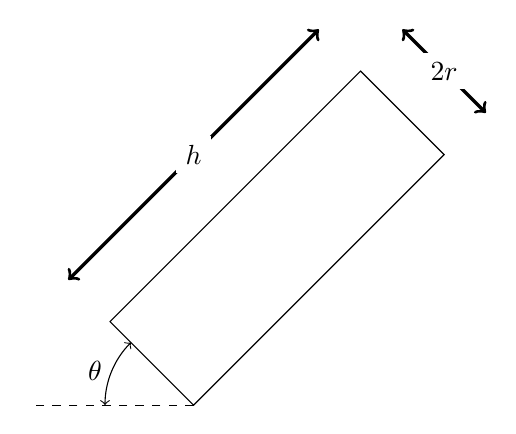
\begin{tikzpicture}[scale=1.5]
        %% cylinder
        \draw (0,0) -- ++(45:3) -- ++(135:1) -- ++(225:3) -- cycle;
        %% Vectors
        \draw[very thick,<->] (45:3.5) -- ++(135:1) node[anchor=center,pos=0.5,fill=white] {$2r$};
        \draw[very thick,<->] (135:1.5) -- ++(45:3) node[anchor=center,pos=0.5,fill=white] {$h$};
        %% horizontal
        \draw[dashed] (0,0) -- (-1.4,0);
        \draw[<->] (-0.75,0) arc (180:135:0.75) node[pos=0.5,anchor=east] {$\theta$};
    \end{tikzpicture}
    \end{center}
    At what angle $\theta$ will the cylinder of height $h$ and radius $r$ be in unstable equilibrium?
    \begin{multicols}{2}
    \begin{choices}
        \wrongchoice{$\theta=\sin^{-1}\left(\dfrac{2r}{h}\right)$}
        \wrongchoice{$\theta=\cos^{-1}\left(\dfrac{2r}{h}\right)$}
      \correctchoice{$\theta=\tan^{-1}\left(\dfrac{2r}{h}\right)$}
        \wrongchoice{$\theta=\sin^{-1}\left(\dfrac{r}{h}\right)$}
        \wrongchoice{$\theta=\tan^{-1}\left(\dfrac{r}{h}\right)$}
    \end{choices}
    \end{multicols}
\end{question}
}

\element{serway-mc}{
\begin{question}{serway-ch12-q18}
    Pairs of forces of equal magnitude act on identical cylinders as shown in the figures.
    In which example is the cylinder in translational and rotational equilibrium?
    \begin{multicols}{2}
    \begin{choices}
        \AMCboxDimensions{down=-1.5cm}
        \wrongchoice{
            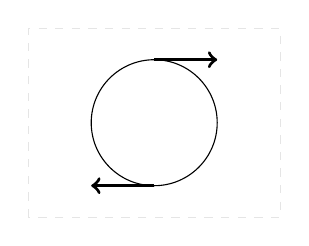
\begin{tikzpicture}[scale=0.8]
                \draw[dashed,white!90!black] (-2,-1.5) rectangle (2,1.5);
                \draw (0,0) circle (1cm);
                %% Vectors
                \draw[very thick,->] (0,+1) -- ++(0:1cm);
                \draw[very thick,->] (0,-1) -- ++(180:1cm);
            \end{tikzpicture}
        }
        %% ANS is B
        \correctchoice{
            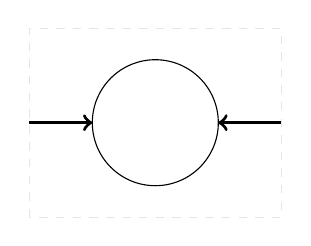
\begin{tikzpicture}[scale=0.8]
                \draw[dashed,white!90!black] (-2,-1.5) rectangle (2,1.5);
                \draw (0,0) circle (1cm);
                %% Vectors
                \draw[very thick,<-] (+1,0) -- ++(0:1cm);
                \draw[very thick,<-] (-1,0) -- ++(180:1cm);
            \end{tikzpicture}
        }
        \wrongchoice{
            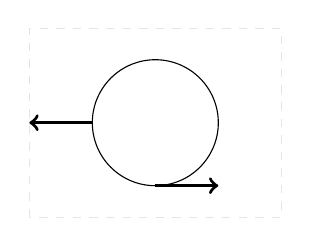
\begin{tikzpicture}[scale=0.8]
                \draw[dashed,white!90!black] (-2,-1.5) rectangle (2,1.5);
                \draw (0,0) circle (1cm);
                %% Vectors
                \draw[very thick,->] (-1,0) -- ++(180:1cm);
                \draw[very thick,->] (0,-1) -- ++(0:1cm);
            \end{tikzpicture}
        }
        \wrongchoice{
            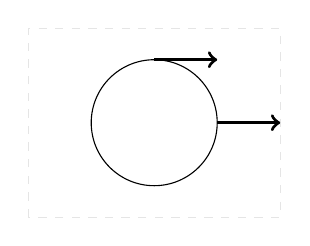
\begin{tikzpicture}[scale=0.8]
                \draw[dashed,white!90!black] (-2,-1.5) rectangle (2,1.5);
                \draw (0,0) circle (1cm);
                %% Vectors
                \draw[very thick,->] (0,+1) -- ++(0:1cm);
                \draw[very thick,->] (+1,0) -- ++(0:1cm);
            \end{tikzpicture}
        }
        \wrongchoice{
            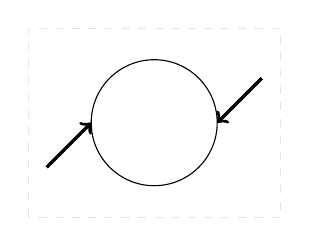
\begin{tikzpicture}[scale=0.8]
                \draw[dashed,white!90!black] (-2,-1.5) rectangle (2,1.5);
                \draw (0,0) circle (1cm);
                %% Vectors
                \draw[very thick,<-] (+1,0) -- ++(45:1cm);
                \draw[very thick,<-] (-1,0) -- ++(225:1cm);
            \end{tikzpicture}
        }
    \end{choices}
    \end{multicols}
\end{question}
}

\element{serway-mc}{
\begin{question}{serway-ch12-q19}
    Angie says that an object is in equilibrium if the net torques about the center of mass is zero.
    Robbie says that an object is in equilibrium if the sum of external forces is zero.
    Which one, if either, is correct?
    \begin{choices}
        \wrongchoice{Both are correct: an object is in equilibrium if either condition holds.}
        \wrongchoice{Neither is correct: both conditions must hold simultaneously.}
      \correctchoice{Neither is correct: the net external force and the net external torque about any axis must be zero.}
        \wrongchoice{Neither is correct: an object is in equilibrium only if its velocity is zero in all coordinate systems.}
        \wrongchoice{Both are correct: if the sum of the external forces is zero, the net torque about any axis is automatically zero, and vice versa.}
    \end{choices}
\end{question}
}

\element{serway-mc}{
\begin{questionmult}{serway-ch12-q20}
    The center of gravity of an object is at the same position as the center of mass when:
    \begin{choices}
      \correctchoice{the object is so far from any mass that $\vec{g}=0$.}
      \correctchoice{the object is located in a region where $\vec{g}$ is uniform over the entire object.}
        \wrongchoice{the object is as large as the body that exerts the gravitational force on it.}
        %\wrongchoice{any of the conditions above is satisfied.}
        %\correctchoice{only (a) or (b) above is satisfied.}
    \end{choices}
\end{questionmult}
}

\element{serway-mc}{
\begin{question}{serway-ch12-q21}
    An object of mass $m$ is suspended by two coplanar wires,
        as shown below.
    \begin{center}
    \begin{tikzpicture}
        %% Ceiling
        \draw[thick] (-4,0) -- (4,0);
        \node[anchor=south,fill,pattern=north east lines,minimum width=8cm, minimum height=0.1cm] at (0,0) {};
        %% mass
        \node[draw,fill=white!90!black,minimum width=2cm,minimum height=1cm,anchor=north] (A) at (0,-1) {$m$};
        %% strings east
        \draw (A.north east) -- ++(30:2);
        \draw[dashed] (A.north east) -- ++(0:2);
        \draw[<->] (A.north east) ++(0:1.5) arc(0:30:1.5) node[pos=0.5,anchor=west] {\ang{30}};
        %% strings west
        \draw (A.north west) -- ++(150:2);
        \draw[dashed] (A.north west) -- ++(180:2);
        \draw[<->] (A.north west) ++(180:1.5) arc(180:150:1.5) node[pos=0.5,anchor=east] {\ang{30}};
    \end{tikzpicture}
    \end{center}
    The tension in each wire has a magnitude given by:
    \begin{multicols}{3}
    \begin{choices}
        \wrongchoice{$\dfrac{\sqrt{2}}{2} mg$}
        \wrongchoice{$\dfrac{\sqrt{3}}{2} mg$}
        \wrongchoice{$\dfrac{1}{2} mg$}
      \correctchoice{$mg$}
        \wrongchoice{$\sqrt{2} mg$}
    \end{choices}
    \end{multicols}
\end{question}
}

\element{serway-mc}{
\begin{question}{serway-ch12-q22}
    Sebastian has drawn a free-body diagram for a ladder of mass $m$ leaning against a frictionless wall.
    His diagram is shown below.
    \begin{center}
    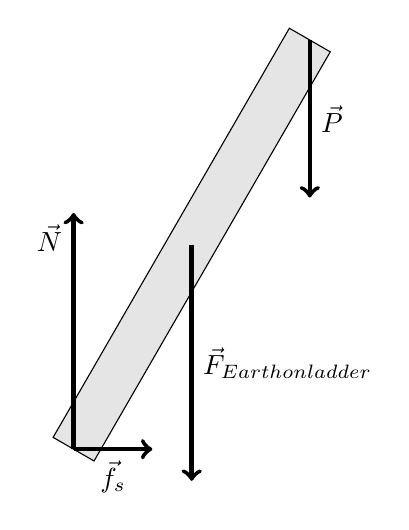
\begin{tikzpicture}
        %% Block
        \draw[fill=white!90!black,rotate around={-30:(0,0)}] (-0.3,0) rectangle (0.3,6);
        %% Vectors
        \draw[ultra thick,->] (0,0) -- (1,0) node[anchor=north,pos=0.5] {$\vec{f}_s$};
        \draw[ultra thick,->] (0,0) -- (0,3) node[anchor=north east,pos=1.0] {$\vec{N}$};
        \draw[ultra thick,->] (60:3) -- ++(270:3) node[anchor=west,pos=0.5] {$\vec{F}_{\text{Earth on ladder}}$};
        \draw[ultra thick,->] (60:6) -- ++(270:2) node[anchor=west,pos=0.5] {$\vec{P}$};
    \end{tikzpicture}
    \end{center}
    \begin{choices}
        \wrongchoice{$\vec{f}_s$ is in the wrong direction.}
        \wrongchoice{$\vec{\mathbf{P}}$ should be directed upwards, not down.}
      \correctchoice{$\vec{\mathbf{P}}$ should be perpendicular to the wall, not parallel to it.}
        \wrongchoice{$\vec{\mathbf{N}}$ should be down into the floor for f s to have the given direction.}
        \wrongchoice{$\vec{\mathbf{P}}$ is correct, but there should also be a force perpendicular to the wall.}
    \end{choices}
\end{question}
}

\element{serway-mc}{
\begin{question}{serway-ch12-q23}
    Stress is proportional to strain means that:
    \begin{choices}
      \correctchoice{stress = constant $\times$ strain.}
        \wrongchoice{stress = (constant\textsubscript{1} $\times$ strain) + constant\textsubscript{2}.}
        \wrongchoice{stress = constant $\div$ strain.}
        \wrongchoice{stress = (constant\textsubscript{1} $\div$ strain) + constant\textsubscript{2}.}
        \wrongchoice{stress $\times$ strain = constant.}
    \end{choices}
\end{question}
}

\element{serway-mc}{
\begin{question}{serway-ch12-q24}
    A mobile is made of identical objects of mass $m$ suspended so that the lowest row has one object,
        the row above two objects, and the row above three objects.
    All the strings are at \ang{45} angles.
    \begin{center}
    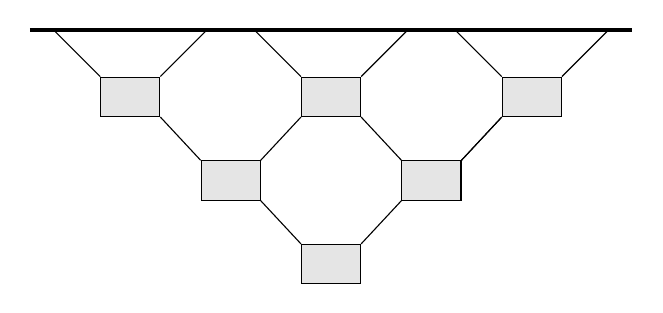
\begin{tikzpicture}[scale=0.85]
        %% Ceiling
        \draw[ultra thick] (-4.5,0) -- (4.5,0);
        %\node[anchor=south,fill,pattern=north east lines,minimum width=9cm, minimum height=0.1cm] at (0,0) {};
        %% blocks top row
        \node[draw,fill=white!90!black,minimum width=0.75cm,minimum height=0.50cm,anchor=center] (A) at (-3,-1) {};
        \node[draw,fill=white!90!black,minimum width=0.75cm,minimum height=0.50cm,anchor=center] (B) at (0,-1) {};
        \node[draw,fill=white!90!black,minimum width=0.75cm,minimum height=0.50cm,anchor=center] (C) at (3,-1) {};
        %% blocks middle row
        \node[draw,fill=white!90!black,minimum width=0.75cm,minimum height=0.50cm,anchor=center] (D) at (-1.5,-2.25) {};
        \node[draw,fill=white!90!black,minimum width=0.75cm,minimum height=0.50cm,anchor=center] (E) at (+1.5,-2.25) {};
        %% blocks bottom row
        \node[draw,fill=white!90!black,minimum width=0.75cm,minimum height=0.50cm,anchor=center] (F) at (0,-3.5) {};
        %% top strings
        \draw (A.north west) -- ++(135:1.00);
        \draw (A.north east) -- ++(45:1.00);
        \draw (B.north west) -- ++(135:1.00);
        \draw (B.north east) -- ++(45:1.00);
        \draw (C.north west) -- ++(135:1.00);
        \draw (C.north east) -- ++(45:1.00);
        %% middle strings
        \draw (A.south east) -- (D.north west);
        \draw (B.south west) -- (D.north east);
        \draw (B.south east) -- (E.north west);
        \draw (C.south west) -- (E.north east);
        \draw (C.south west) -- (E.north east);
        %% bottom strings
        \draw (D.south east) -- (F.north west);
        \draw (E.south west) -- (F.north east);
    \end{tikzpicture}
    \end{center}
    What is the tension in the strings connecting the highest row to the ceiling?
    \begin{multicols}{3}
    \begin{choices}
        \wrongchoice{$\dfrac{1}{2}mg$}
        \wrongchoice{$\dfrac{\sqrt{2}}{2}mg$}
        \wrongchoice{$mg$}
        \wrongchoice{$\dfrac{\sqrt{2}}{3}mg$}
      \correctchoice{$\dfrac{3\sqrt{2}}{2}mg$}
    \end{choices}
    \end{multicols}
\end{question}
}

\element{serway-mc}{
\begin{question}{serway-ch12-q25}
    John is carrying a shovelful of snow.
    The center of mass of the \SI{3.00}{\kilo\gram} of snow he is holding is \SI{15.0}{\centi\meter} from the end of the shovel.
    He is pushing down on the opposite end of the shovel with one hand and holding it up \SI{30.0}{\centi\meter} from that end with his other hand.
    Ignore the mass of the shovel.
    Sarah says that his hand pushing down on the shovel must be exerting a greater force than the hand pushing up.
    James says it is just the reverse.
    Which one, if either, is correct?
    \begin{choices}[o]
        \wrongchoice{Sarah, because the hand pushing down must exert a greater force to match the torque exerted by the snow.}
        \wrongchoice{James, because, depending on the location of the axis of rotation, the hand pushing down can counteract the torque exerted by the snow.}
        \wrongchoice{James, because the hand pushing up must exert a force that equals the sum of the force of the hand pushing down and the weight of the snow.}
      \correctchoice{James, because both (b) and (c) above are correct.}
        \wrongchoice{Neither, because the hands exert forces of equal magnitudes.}
    \end{choices}
\end{question}
}


\endinput



